% Copyright 2024 by Marcos Laureano (marcos.laureano@ifpr.edu.br)
% This file may be distributed and/or modified
%
% 1. under the LaTeX Project Public License and/or
% 2. under the GNU Public License.

\documentclass{standalone}

\usepackage{tikz}
\usetikzlibrary{arrows,decorations.pathmorphing,positioning,fit,petri}
\usetikzlibrary{calc,intersections,through,backgrounds,graphs}
\usetikzlibrary{patterns,decorations.pathreplacing}

\begin{document}


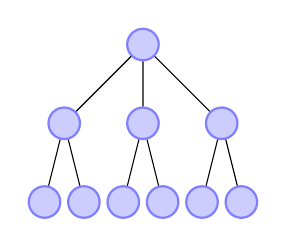
\begin{tikzpicture}
 [
  level/.style={sibling distance = 1cm/#1,level distance = 1cm},
  place/.style={circle,draw=blue!50,fill=blue!20,thick, inner sep=0pt,minimum size=4mm},
 ]
  \node [place] {}
     child{ node [place] {} 
            child{ node [place] {}}
            child{ node [place] {}}
            %child{ node [place] {3}}
            %child{ node [place] {3}}
    }
    child{ node [place] {}
            child{ node [place] {}}
            child{ node [place] {}}
            %child{ node [place] {}}
            %child{ node [place] {}}
    }
    child{ node [place] {}
							child{ node [place] {}}
							child{ node [place] {}}
    }
    %child{ node [place] {} }
	
; 
\end{tikzpicture}
\end{document}